\chapter{Essential Algebra}
\paragraph{} Meanwhile, Duckie and Güs's various competitions made the goose authorities a bit confused. Because of Duckie and Güs's "she-goose-igans", they lost track of where Duckie was. They decided that they needed to review their records of Duckie and Güs's locations, and try to figure out what they were doing on the 5th day. 
\vfill
\pagebreak
%Equality
\subchapter{Equality}
{Because Duckie and Güs were travelling together, they were always at the same position at any time.}
{Güs's position = Duckie's position. Duckie's position was P4, so Güs's position was also P4}
{When two things are the same, we write this in mathematics as "="}
{\begin{tikzpicture}
    \coordinate (A) at (0,0);
    \coordinate (B) at (0,6.4);
    \coordinate (Ap) at (2,0);
    \coordinate (Bp) at (2,6.4);
    
    \node [inner sep=0pt] at (B) {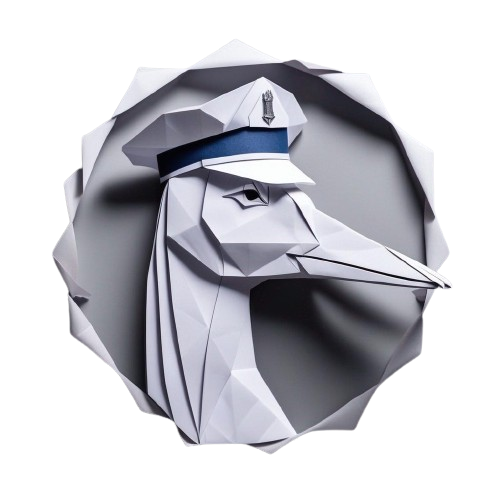
\includegraphics[height=0.8cm]{Gus}};
    \draw[->,ultra thick,red, decorate, decoration={random steps,segment length=3pt,amplitude=0.2pt}] (A) -- (B) node[midway, left] {38 km};
    \node [inner sep=0pt] at (Bp) {
\includegraphics[height=0.8cm]{DuckieGami}};
    \draw[->,ultra thick,blue, decorate, decoration={random steps,segment length=3pt,amplitude=0.2pt}] (Ap) -- (Bp) node[midway, left] {38 km};
\end{tikzpicture}}
%The Equality Rule
\subchapter{The Equality Rule}
{The goose authorities, having trained Güs in the police academy, knew he was a very fast flyer. In fact, he had won the village racing competition for the past three years! Because Duckie and Güs were travelling together, they realized that every time Güs had flown ahead of Duckie, Duckie had to increase his position by the same amount to keep up.}
{Duckie's position + $\Delta$x = Güs's position + $\Delta$x}
{What happens to one side of an equation must happen to the other side so that they are still equal.}
{\begin{tikzpicture}
    \coordinate (A) at (0,0);
    \coordinate (B) at (0,6.4);
    \coordinate (C) at (0,9.4);
    \coordinate (Ap) at (2,0);
    \coordinate (Bp) at (2,6.4);
    \coordinate (Cp) at (2,9.4);
    
    \node [inner sep=0pt] at (C) {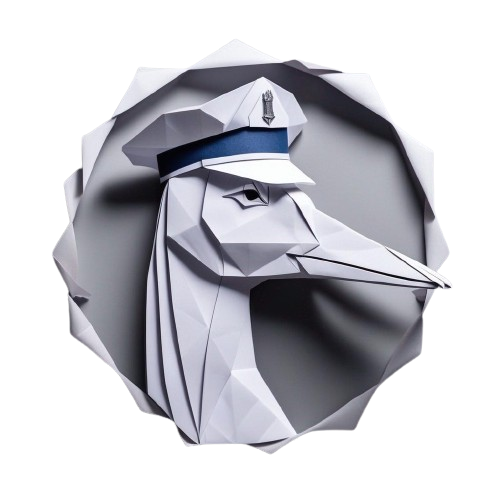
\includegraphics[height=0.8cm]{Gus}};
    \draw[->,ultra thick,red, decorate, decoration={random steps,segment length=3pt,amplitude=0.2pt}] (A) -- (B) node[midway, left] {38 km};
    \draw[->,ultra thick,orange, decorate, decoration={random steps,segment length=3pt,amplitude=0.2pt}] (B) -- (C) node[midway, left] {24 km};
    \node [inner sep=0pt] at (Cp) {
\includegraphics[height=0.8cm]{DuckieGami}};
    \draw[->,ultra thick,blue, decorate, decoration={random steps,segment length=3pt,amplitude=0.2pt}] (Ap) -- (Bp) node[midway, left] {38 km};
    \draw[->,ultra thick,orange, decorate, decoration={random steps,segment length=3pt,amplitude=0.2pt}] (Bp) -- (Cp) node[midway, left] {24 km};
    
    \draw [decorate, decoration = {calligraphic brace,mirror, raise=10pt,amplitude=5pt}] (Ap) -- (Cp) node[midway, right, xshift=0.5cm,line width=3pt] {62 km};
\end{tikzpicture}}
%Commutativity
\subchapter{Variables}
{The goose authorities were still a bit confused about Duckie and Güs's progress. They knew that there were 4 competitions, and that they started at 38 km. They also knew that they ended at 62 km. How much did they travel on average in each competition?}
{\begin{center} 4x + 38 = 62 \linebreak 4x + 38 = 62 - 38 \linebreak $\frac{4x}{4}$ = $\frac{24}{4}$ \linebreak x = $8$  \end{center}}
{Letters and Symbols can be used to represent a number which isn’t already known, such as X. 2x + 3 = 6 means that 2*(some number) + 3 = 6.}
{\begin{tikzpicture}
    \coordinate (A) at (0,0);
    \coordinate (B) at (0,1);
    \coordinate (C) at (0,2);
    \coordinate (D) at (0,3);
    \coordinate (E) at (0,4);
    \coordinate (F) at (0,10);
    \coordinate (Ap) at (1.5,0);
    \coordinate (Bp) at (1.5,1);
    \coordinate (Cp) at (1.5,2);
    \coordinate (Dp) at (1.5,3);
    \coordinate (Ep) at (1.5,4);
    \coordinate (Fp) at (1.5,10);
    \coordinate (Af) at (3.4,0);
    \coordinate (Bf) at (3.4,1);
    \node [inner sep=0pt] at (F) {
\includegraphics[height=0.8cm]{DuckieGami}};
    \draw[->,ultra thick,blue, decorate, decoration={random steps,segment length=3pt,amplitude=0.2pt}] (A) -- (B) node[midway, left] {? km};
    \draw[->,ultra thick,blue, decorate, decoration={random steps,segment length=3pt,amplitude=0.2pt}] (B) -- (C) node[midway, left] {? km};
    \draw[->,ultra thick,blue, decorate, decoration={random steps,segment length=3pt,amplitude=0.2pt}] (C) -- (D) node[midway, left] {? km};
    \draw[->,ultra thick,blue, decorate, decoration={random steps,segment length=3pt,amplitude=0.2pt}] (D) -- (E) node[midway, left] {? km};
    \draw[->,ultra thick,green, decorate, decoration={random steps,segment length=3pt,amplitude=0.2pt}] (E) -- (F) node[midway, left] {38 km};
    \draw [decorate, decoration = {calligraphic brace, raise=35pt,amplitude=5pt}] (A) -- (F) node[midway, left, xshift=-1.5cm,line width=3pt] {62 km};
    
    \draw[->,ultra thick,blue, decorate, decoration={random steps,segment length=3pt,amplitude=0.2pt}] (Ap) -- (Bp) node[midway, left] {? km};
    \draw[->,ultra thick,blue, decorate, decoration={random steps,segment length=3pt,amplitude=0.2pt}] (Bp) -- (Cp) node[midway, left] {? km};
    \draw[->,ultra thick,blue, decorate, decoration={random steps,segment length=3pt,amplitude=0.2pt}] (Cp) -- (Dp) node[midway, left] {? km};
    \draw[->,ultra thick,blue, decorate, decoration={random steps,segment length=3pt,amplitude=0.2pt}] (Dp) -- (Ep) node[midway, left] {? km};
    \draw[->,ultra thick,red, decorate, decoration={random steps,segment length=3pt,amplitude=0.2pt}] (Fp) -- (Ep) node[midway, left] {-38 km};
    \draw [decorate, decoration = {calligraphic brace,mirror, raise=10pt,amplitude=5pt}] (Ap) -- (Ep) node[midway, right, xshift=0.5cm,line width=3pt] {24 km};
    
    \draw[->,ultra thick,blue, decorate, decoration={random steps,segment length=3pt,amplitude=0.2pt}] (Af) -- (Bf) node[midway, left] {8 km};
\end{tikzpicture}}